\chapter{Παράδειγμα Χρήσης Βιβλιοθήκης}
\label{chap:Demo}

Στην παρούσα ενότητα θα χρησιμοποιηθεί η βιβλιοθήκη για την 
προσθήκη επιπλέον υπηρεσιών και διαδικασιών. Στόχος είναι να 
παρουσιαστεί ο τρόπος και η ευκολία με την οποία μπορούν να 
κατασκευαστούν πολύπλοκες διαδικασίες με την αρχιτεκτονική που 
προτείνουμε.

Στο σύστημα Θα προστεθεί λειτουργικότητα που αφορά τον 
διαμοιρασμό αρχείων μεταξύ των peer του δικτύου. Στις ακόλουθες 
υποενότητες θα αναλυθεί το πρόβλημα και τι προσθήκες απαιτούνται. Επίσης 
αναλύεται ο τρόπος με τον οποίο θα γίνουν αυτές οι προσθήκες.

\section{Ανάλυση Προβλήματος}

Ο στόχος όπως αναφέρθηκε είναι η προσθήκη λειτουργικότητας 
διαμοιρασμού αρχείων. Από αυτό συνεπάγεται πως ένας peer πρέπει να έχει 
μια δομή όπου θα κρατά στοιχεία για τα αρχεία τα οποία είναι 
αποθηκευμένα τοπικά. Κάθε αρχείο αντιστοιχεί σε ένα συγκεκριμένο κλειδί 
του δικτύου. Βάσει αυτού μπορεί να αναζητηθεί και να βρεθεί ο peer που 
κατέχει το αρχείο.

Πρέπει να εισαχθούν οι απαραίτητες αφαιρέσεις ώστε να 
παρουσιαστεί το δίκτυο ως ένας ενιαίος αποθηκευτικός χώρος. Βασικές 
λειτουργίες είναι η αποθήκευση ενός αρχείου στο δίκτυο και η αναζήτηση. 
Η αναζήτηση αρχείου είτε θα επιστρέψει τον κάτοχο peer σήμα ότι υπάρχει 
στο δίκτυο είτε τίποτα.

Μια βασική λειτουργία που πρέπει να υπάρχει σε ένα σύστημα διαμοιρασμού 
αρχείων είναι η δυνατότητα μεταφοράς αρχείων από μεταξύ των peer. Πέρα 
από την λήψη του αρχείου είναι απαραίτητη η αναφορά προόδου λήψης καθώς 
και η κατάσταση της (ανενεργό, αναμονή, λήψη). 

\begin{figure}[htbp]
  \begin{center}
    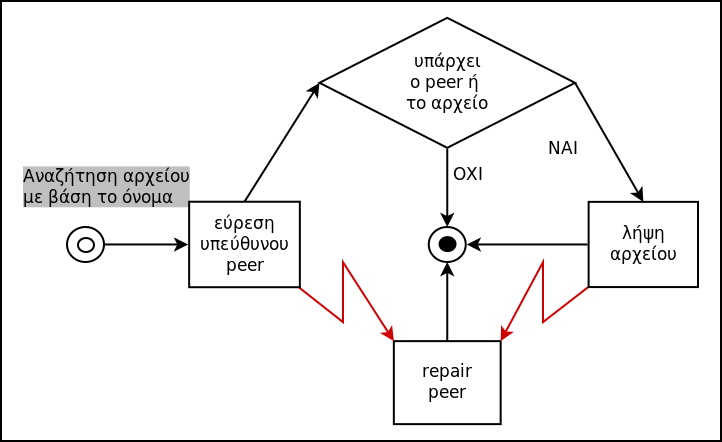
\includegraphics[width=0.9\textwidth]{Figures/Demo/Workflow.png}
  \end{center}
  \caption{Διάγραμμα ροής αναζήτησης και λήψης αρχείου}
  \label{fig:Workflow}
\end{figure}

Τέλος η διαδικασία που είναι άμεσα χρήσιμη στο επίπεδο εφαρμογής 
είναι η αναζήτηση ενός αρχείου και η λήψη του σε περίπτωση που υπάρχει. 
Παραπάνω φαίνεται το διάγραμμα ροής αυτής της διεργασίας. Σε περίπτωση 
που ανακαλυφθεί μια αποτυχία κατά την εκτέλεση της τότε πρέπει να 
επιλυθεί.

\section{Υλοποίηση}

Από την προηγούμενη ανάλυση διακρίνουμε δύο υπηρεσίες που αφορούν τον 
αποθηκευτικό χώρο του δικτύου (Storage Service) και την μεταφορά αρχείων 
μεταξύ των peer (File Transfer Service). Η σύνθεση αυτών των δυο 
συνιστούν την διαδικασία αναζήτησης και λήψης (Download File Process). 
Για απλότητα σε κάθε peer υπάρχει ένας φάκελος όπου χρησιμοποιείται ως 
αποθηκευτικός χώρος για τα διαμοιραζόμενα αρχεία και άλλος ένας φάκελος 
όπου αποθηκεύονται τα αρχεία που από την υπηρεσία λήψης.

Σύμφωνα με την ανάλυση της αρχιτεκτονικής για να προστεθούν οι υπηρεσίες 
στο σύστημα αρκεί να υλοποιηθούν τρεις συγκεκριμένες διεπαφές/κλάσεις. Η 
κλάση AbstractModule περιγράφει την παραμετροποίηση της υπηρεσίας, ποιες 
υλοποιήσεις αντιστοιχούν σε ποιες διεπαφές. Η διεπαφή Provider είναι 
απαραίτητη για την παροχή αντικειμένων της υπηρεσίας. Μάλιστα, μέσω των 
Provider καθορίζεται και ο κύκλος ζωής της. Ο τρόπος αρχικοποίησης και 
εγκατάστασης της υπηρεσίας στο σύστημα γίνεται δια μέσου της διεπαφής 
ServiceRegistration. Τέλος, είναι αναγκαίο ο ορισμός ενός annotation ο 
οποίος χρησιμοποιείται για τον καθορισμό ποιας υλοποίησης της 
ServiceRegistration θα χρησιμοποιηθεί δεδομένου ότι υπάρχουν και άλλες 
υπηρεσίες.

Από εκεί και πέρα χρειάζεται μια διεπαφή που θα περιγράφει και θα 
εκθέτει την λειτουργικότητα της υπηρεσίας. Απαιτείται η υλοποίηση του 
κομματιού που αφορά την CORBA. Τέλος, εσωτερικά σε κάθε module υπηρεσίας 
χρειάζεται να ακολουθηθεί μια δομή όπου θα διευκολύνει την επέκταση και 
την τροποποίηση της συμπεριφοράς αυτής.

\begin{figure}[htbp]
  \begin{center}
    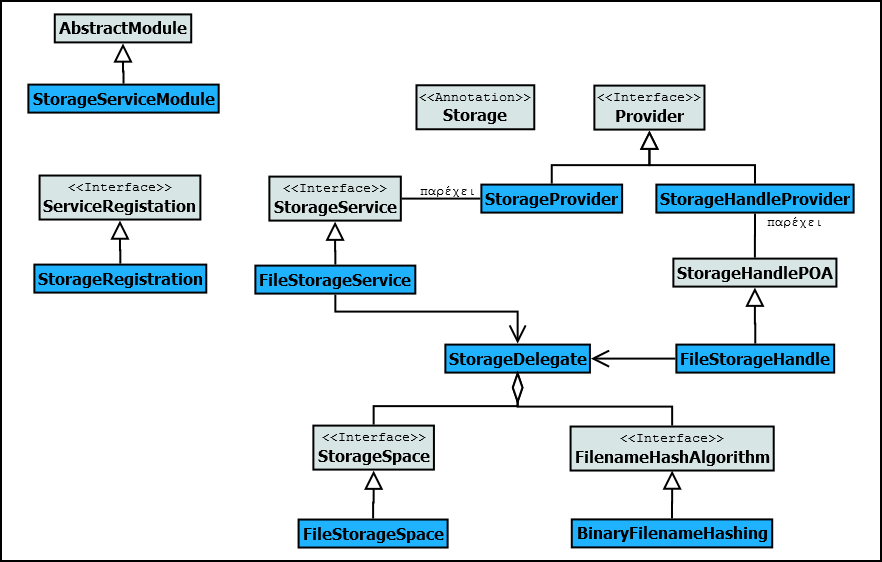
\includegraphics[width=0.95\textwidth]{Figures/Demo/StorageService_ClassDiagram.png}
  \end{center}
  \caption{Διάγραμμα κλάσεων υπηρεσίας StorageService}
  \label{fig:StorageService}
\end{figure}

\paragraph{Υλοποίηση StorageService και FileTransferService.} 
Στην εικόνα \ref{fig:StorageService} φαίνεται το διάγραμμα κλάσεων 
της υπηρεσίας StorageService. Μπορούμε να δούμε τα αντικείμενα που 
υλοποιούν ή επεκτείνουν τις απαραίτητες διεπαφές/κλάσεις όπως έχει 
περιγραφεί παραπάνω. Οι κλάσεις StorageHandlePOA έχει παραχθεί από 
την idl και αφορά την CORBA. Παρέχεται Provider και για αυτή την 
διεπαφή. Στην εικόνα \ref{fig:FileTransferService} φαίνεται το 
διάγραμμα κλάσεων της υπηρεσίας FileTransferService. Ακολουθείται 
αντίστοιχη λογική.

\begin{figure}[htbp]
  \begin{center}
    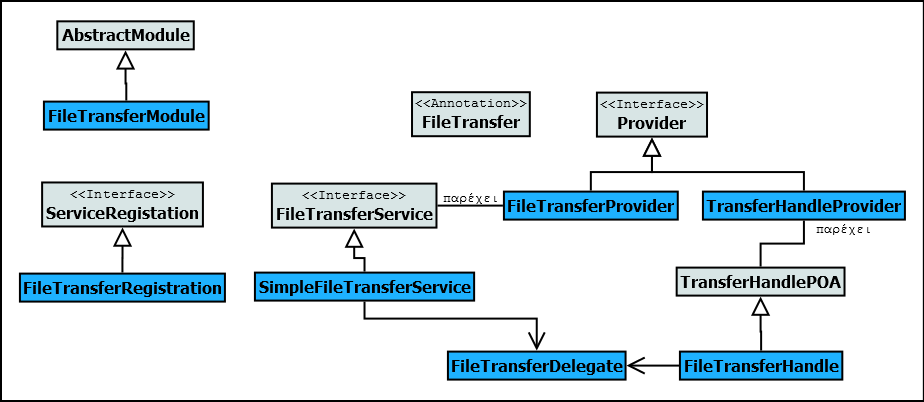
\includegraphics[width=0.95\textwidth]{Figures/Demo/FileTransferService_ClassDiagram.png}
  \end{center}
  \caption{Διάγραμμα κλάσεων υπηρεσίας FileTransferService}
  \label{fig:FileTransferService}
\end{figure}

\paragraph{Υλοποίηση DownloadFileProcess.}
Αυτό που μένει είναι η υλοποίηση της διαδικασίας 
DownloadFileProcess. Το διάγραμμα κλάσεων φαίνεται στην εικόνα 
\ref{fig:DownloadFileProcess}. Φαίνεται και η χρήση της υπηρεσίας 
επιδιόρθωσης RepairService που καταστά την διαδικασία fault-tolerant.

\begin{figure}[htbp]
  \begin{center}
    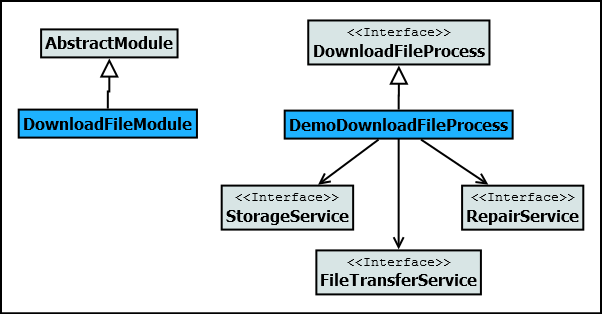
\includegraphics[width=0.9\textwidth]{Figures/Demo/DownloadFileProcess_ClassDiagram.png}
  \end{center}
  \caption{Διάγραμμα κλάσεων διαδικασίας DownloadFileProcess}
  \label{fig:DownloadFileProcess}
\end{figure}

Στην εικόνα \ref{fig:DownloadFile_Sequence} φαίνεται το διάγραμμα 
ακολουθίας της διαδικασία όταν καλείται από τον χρήστη. Φαίνεται ξεκάθαρα 
πώς τα αντικείμενα σε επίπεδο διαδικασίας αλληλεπιδρούν. Συγκεκριμένα φαίνεται 
η περίπτωση όπου το αρχείο υπάρχει σε κάποιον peer το δικτύου ο οποίος 
και επιστρέφεται όταν τερματίζει η εκτέλεση της υπηρεσίας 
StorageService. Η διαδικασία επιστρέφει στον χρήστη την κατάσταση στην 
οποία τερμάτισε. Οι καταστάσεις που έχουν οριστεί στην διεπαφή είναι 
FILE\_NOT\_FOUND, NETWORK\_ERROR και FILE\_DOWNLOADED. Επίσης, φαίνεται 
και ο κύκλος ζωής των υπηρεσιών αυτών. Σε νέα αίτηση θα κατασκευαστούν 
εκ νέου τα αντικείμενα. Κάτι αντίστοιχο συμβαίνει όταν ο peer δέχεται 
αιτήσεις για εξυπηρέτηση υπηρεσιών. Η διαφορά είναι ότι εκεί τα 
αντικείμενα που αφορούν την CORBA είναι ίδια μέχρι τον τερματισμό του 
peer.

\begin{figure}[htbp]
  \begin{center}
    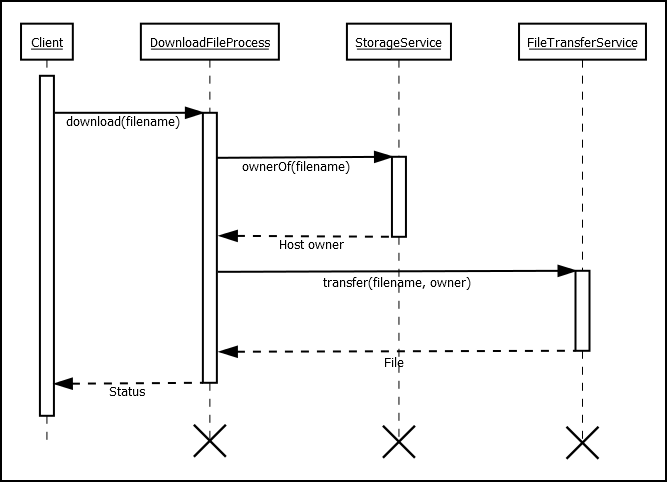
\includegraphics[width=0.9\textwidth]{Figures/Demo/DownloadFileProcess_Sequence.png}
  \end{center}
  \caption{Διάγραμμα ακολουθίας της διαδικασίας DownloadFileProcess}
  \label{fig:DownloadFile_Sequence}
\end{figure}
